\section{Deep Learning Models: Autoencoder Architectures}

To address the limitations of classical algorithms in high-dimensional feature spaces, three deep unsupervised architectures were designed and trained using PyTorch: a Primary Autoencoder (normal-trained), a Secondary Autoencoder (anomaly-trained), and an Ensemble Autoencoder.

\subsection{Primary Autoencoder (Normal-Trained)}
The primary autoencoder is designed for reconstruction-error-based anomaly detection. It is trained exclusively on normal (benign) network traffic ($\mathbf{X}_{\text{train}}$ where $y_{\text{train}} = 0$) to learn a compact representation of standard network behavior. The model comprises an encoder $f_{\theta}$ and a decoder $g_{\phi}$, both parameterized by fully connected feedforward networks:

\begin{equation}
  \mathbf{z} = f_{\theta}(\mathbf{x}) = \sigma(\mathbf{W}_3 \sigma(\mathbf{W}_2 \sigma(\mathbf{W}_1 \mathbf{x} + \mathbf{b}_1) + \mathbf{b}_2) + \mathbf{b}_3)
\end{equation}
\begin{equation}
  \mathbf{\hat{x}} = g_{\phi}(\mathbf{z}) = \sigma(\mathbf{W}_6 \sigma(\mathbf{W}_5 \sigma(\mathbf{W}_4 \mathbf{z} + \mathbf{b}_4) + \mathbf{b}_5) + \mathbf{b}_6)
\end{equation}

where $\sigma$ denotes the Rectified Linear Unit (ReLU) activation function, and $\mathbf{x} \in \mathbb{R}^{70}$ represents the scaled input. The network contracts the input to a low-dimensional bottleneck space ($\mathbb{R}^{70} \to \mathbb{R}^{32} \to \mathbb{R}^{16} \to \mathbb{R}^8$), regularizing the model to prevent identity mapping, before reconstructing the output ($\mathbb{R}^8 \to \mathbb{R}^{16} \to \mathbb{R}^{32} \to \mathbb{R}^{70}$). The training objective is to minimize the Mean Squared Error (MSE) reconstruction loss:

\begin{equation}
  \mathcal{L}_{\text{MSE}}(\theta, \phi) = \frac{1}{N} \sum_{i=1}^N \|\mathbf{x}^{(i)} - \mathbf{\hat{x}}^{(i)}\|^2
\end{equation}

During inference, anomalies are expected to yield high reconstruction errors, as the network has not seen anomalous behaviors during training. The anomaly score is defined as $s(\mathbf{x}) = \|\mathbf{x} - \mathbf{\hat{x}}\|^2$. A sample is classified as anomalous if $s(\mathbf{x}) > \tau_{\text{primary}}$, where $\tau_{\text{primary}}$ is set to the 80th percentile of the validation reconstruction error.

\subsection{Secondary Autoencoder (Anomaly-Trained)}
Following the complementary-signal paradigm, a secondary autoencoder was implemented with an identical encoder-decoder structure but trained exclusively on anomalous (attack) traffic ($y_{\text{train}} = 1$). This model learns the shared statistical features of malicious network behaviors. 

Because it learns the patterns of attacks, anomalous samples yield low reconstruction errors, whereas benign samples produce high reconstruction errors. The anomaly score is defined as $s_2(\mathbf{x}) = -\|\mathbf{x} - \mathbf{\hat{x}}_2\|^2$ (where $\mathbf{\hat{x}}_2$ is the reconstruction from the secondary autoencoder), so that lower reconstruction errors yield higher anomaly scores. A sample is flagged if $s_2(\mathbf{x}) < \tau_{\text{secondary}}$, where $\tau_{\text{secondary}}$ is set to the 20th percentile.

\subsection{Ensemble Autoencoder}
To maximize detection rates and minimize false negatives (critical in security contexts), an Ensemble Autoencoder was created by combining the primary and secondary models. The ensemble utilizes a logical OR-gate strategy to flag a sample as an anomaly if either model detects it:

\begin{equation}
  \hat{y}_{\text{ensemble}} = \hat{y}_{\text{primary}} \lor \hat{y}_{\text{secondary}}
\end{equation}

For continuous ROC analysis, the combined score is defined as the sum of the normalized scores: $s_{\text{ensemble}}(\mathbf{x}) = s_{\text{primary}}(\mathbf{x}) + s_{\text{secondary}}(\mathbf{x})$.

\subsection{Training Convergence and Analysis}
The training of both autoencoders was performed using the Adam optimizer (learning rate = $0.001$, batch size = $64$). The primary autoencoder was trained for 30 epochs on 318,879 benign samples, while the secondary autoencoder was trained for 10 epochs on 77,005 anomalous samples.

\begin{figure}[ht]
    \centering
    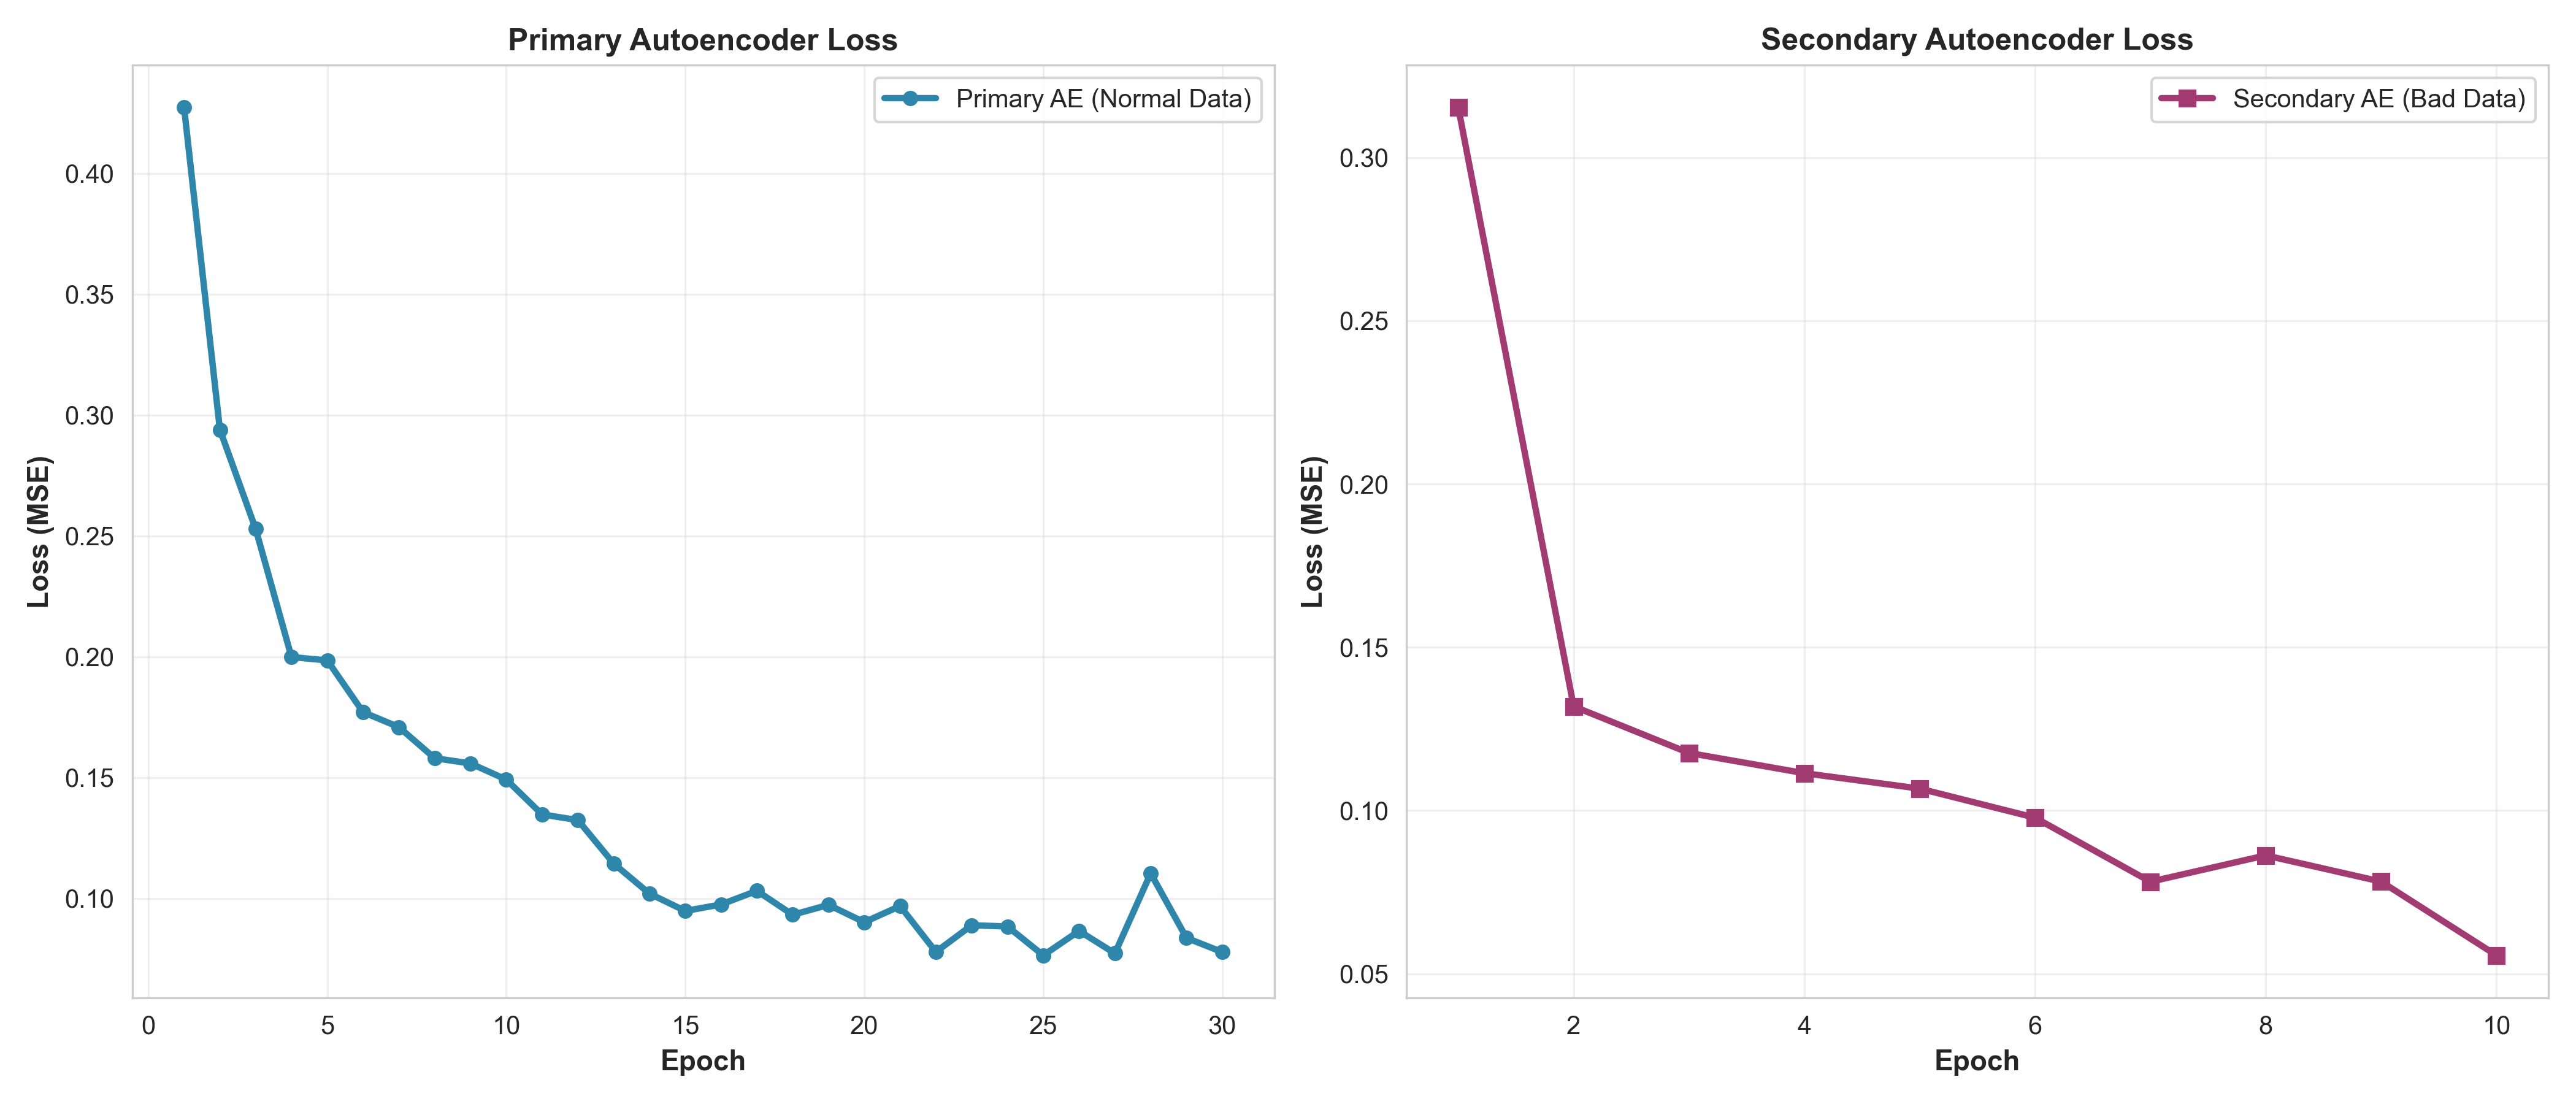
\includegraphics[width=0.75\columnwidth]{images/autoencoder_loss_comparison.png}
    \caption{Training loss (MSE) over epochs for the Primary and Secondary Autoencoders.}
    \label{fig:loss_comparison}
\end{figure}

As shown in Figure~\ref{fig:loss_comparison}, the primary autoencoder converged smoothly, reaching its minimum MSE loss at Epoch 29 ($0.0615$). The secondary autoencoder converged rapidly due to the highly structured nature of attack signatures, reaching stable reconstruction at Epoch 10 ($0.0817$). No overfitting was observed on validation data.

% =============================================================
